\documentclass[]{article}
\usepackage{geometry}
\usepackage{float}
\usepackage{graphicx}
\usepackage[utf8]{inputenc}
\DeclareFixedFont{\ttb}{T1}{txtt}{bx}{n}{9} % for bold
\DeclareFixedFont{\ttm}{T1}{txtt}{m}{n}{9}  % for normal
% Defining colors
\usepackage{color}
\definecolor{deepblue}{rgb}{0,0,0.5}
\definecolor{deepred}{rgb}{0.6,0,0}
\definecolor{deepgreen}{rgb}{0,0.5,0}


\usepackage{listings}

% Python style for highlighting
\newcommand\pythonstyle{\lstset{
		language=Python,
		backgroundcolor=\color{white}, %%%%%%%
		basicstyle=\ttm,
		otherkeywords={self},            
		keywordstyle=\ttb\color{deepblue},
		emph={MyClass,__init__},          
		emphstyle=\ttb\color{deepred},    
		stringstyle=\color{deepgreen},
		commentstyle=\color{red},  %%%%%%%%
		frame=tb,                         
		showstringspaces=false            
	}}
	
	% Python environment
	\lstnewenvironment{python}[1][]
	{
		\pythonstyle
		\lstset{#1}
	}
	{}
\geometry{
	a4paper,
	total={170mm,257mm},
	left=20mm,
	top=20mm,
}
%opening
\title{CAB320 - Artificial Intelligence\\
	Sokoban Solver}
\author{Nathan Perkins}

\begin{document}

\maketitle
\newpage
\section{Computational Environment}
\begin{enumerate}
	\item Operating System: Ubuntu Linux 15.10 was used in the creation of the Sokoban solver and all testing was undertaken in that environment
	\item Python: Python 2.7.10 was used as the basis of the solution to maintain compatibility with the search algorithms already implemented.
	\item Python Dependencies: 
	\begin{enumerate}
		\item Cab320\_search.py: Search algorithm library implemented by Frederic Maire
		\item Cab320\_sokoban.py: Sokoban helper class library implemented by Frederic Maire
		\item Time: Core python library, used to time function calls. No operating system platform dependency.
		\item os: Core python library, used to iterate over files in folders. No operating system platform dependency.
		\item thread + threading: Core python libraries, used to ensure function calls don't go over cut-off time. No operating system platform dependency.
	\end{enumerate}
\end{enumerate}
\section{Elementary Solver}
\subsection{State}
The utilised search algorithms in cab320\_search.py required a state variable be implemented. To keep memory and therefore time to a minimum in searching for the solution space, only the dynamic elements of the puzzle were stored, including the worker and box elements. Static elements, such as the walls, taboo cells and targets were simply stored locally in the SokobanPuzzle class.\\
The state takes the following form\\
\\state[0] = worker : where worker is of the form (x,y). x and y are index co-ordinates
\\state[1] = boxes : where boxes is a tuple of tuples, taking the form (($x_1,y_1$),($x_2,y_2$)...($x_n,y_n$))
 
\subsubsection{Updating State}
In the elementary solver, an action takes the form of possible worker movement. The Cardinal directions dictate the possible actions, however not all directions in a given state are legal. Actions are checked at each state, removing any that would constitute an illegal move. Illegal actions include all of the following and are implemented in the member class function \textit{actions(state)}.
\begin{itemize}
	\item Space occupied by wall.
	\item Space occupied by box if that box can't be pushed in that direction.
	\item Boxes can't be pushed in a direction if there exists no unoccupied space in that direction.
\end{itemize}
If a given action has been deemed legal and selected for the next state, the class member function results(\textit{state,action}) returns the result of that \textit{action}. The worker location stored in \textit{state[0]} is updated with the new location based on current location and \textit{action}. If the new worker position shares a location with a current box position taken from \textit{state[1]} then that box is also updated with a move in the direction of \textit{action}.
\subsection{Heuristics}
The heuristics function, denoted \textit{h(node)} takes a potential \textit{nodes state} variable, then takes the manhattan distance of all boxes to the closest goal state. It then adds the manhattan distance of the worker to the closest box before returning total cost, which is the addition of all mentioned costs. Due to the nature of the sokoban puzzle, a solution will almost never take the form of simply moving the nearest box to the nearest goal position. In all cases it is at most equal to the actual cost of solution. Therefore, the manhattan distance heuristic is an admissible heuristic and suitable to find the lowest cost solution to the puzzle. 
\subsection{Taboo Cells}
There were 2 types of cells identified that were taboo for static taboo cells. Static taboo cells occur due to the walls and other unchanging parts of a puzzle.
\subsubsection{Corner Cells}
 The first type of taboo cell occurs when a corner is encountered on the walls. A worker needs to be on the other side of a box to move it in the chosen direction, therefore once a box moves onto a corner it can't leave. An example of corner cells can be seen in figure \ref{TabooCells}. To compute the taboo cells, each wall location was checked against the remainder of the walls. If the current wall contains any neighbouring wall in a diagonal location, then the two adjacent cells that share both diagonal walls are marked as taboo. After each wall is checked, the list of corner cells is checked to make sure no wall cells or target cells were marker as taboo. 
\subsubsection{Wall Adjacent Cells}
Wall adjacent cells is another type of taboo cell, however this is harder to find. If a box moves adjacent to a wall, where there exists no openings for the worker to get behind the box, it is also a taboo cell. An example of this can be seen in figure \ref{TabooCells}. After checking for taboo corner cells, any cells between two already marked taboo corners is marked taboo if there exists no gap in the wall it borders. The function \textit{static\_taboo\_line(taboo,walls,targets)} computes this. An exception is made if any of the cells in the original line are target states, and taboo cells aren't added in that case. 
\begin{figure}[H]
	\centering
	\caption{Taboo Cells}
	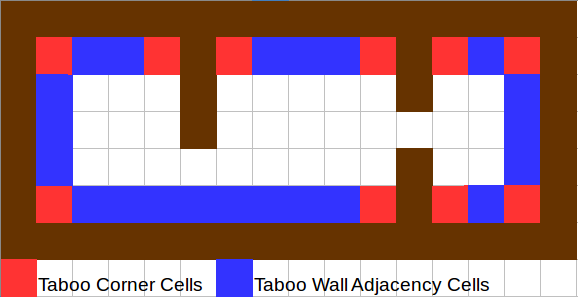
\includegraphics[width=0.5\textwidth]{TabooCells.png}
	\label{TabooCells}
\end{figure}
\section{Macro Solver}
Most features of the elementary solver were carried over to the Macro solver. These include the \textit{state} variables, taboo cells and other static elements of the puzzle. Only 3 things changed between the implementations, the action, its resultant state update, and the heuristic.
\subsection{Actions}
Actions were redefined for the macro actions. Rather than, as in elementary, just moving the worker a single space, all possible spaces in a line are considered. If the worker has an unimpeded "line of sight" to a grid space in one of the cardinal directions it is considered an available action. Furthermore, if "line of sight" is blocked by only 1 box, it can push that box until the box contacts the wall, a taboo cell, or another box. An example of which can be seen below in figure \ref{MacroAction}.
\begin{figure}[H]
	\centering
	\caption{Macro Action Legal Moves}
	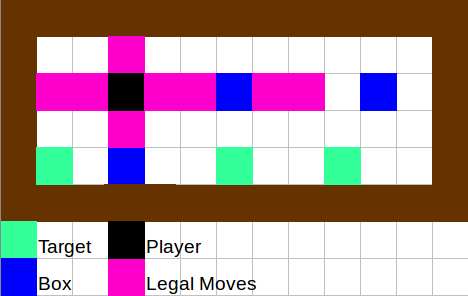
\includegraphics[width=0.5\textwidth]{MacroAction.png}
	\label{MacroAction}
\end{figure}
\newpage
\subsection{Heuristics}
Due to the creation of macro actions, the old heuristics become inadmissible and new heuristics had to be devised. For each box that isn't on target, it computes the manhattan distance of macro moves required to put a box on target. There are 3 potential states it computes for each box.
\begin{enumerate}
	\item The box is on the target, no added cost
	\item The box is directly in line, either x or y with a target, added cost of 1 move
	\item The box is not in line with any targets, added cost of 2 moves
\end{enumerate}
The heuristic adds all these values, then adds a further value for the worker using the same criteria as above, except between worker and box.
\section{Performance}
Both elementary and macro solver only utilise the A* search algorithm instead of the Iterative Deepening A*. Performance was therefore much slower than could be achieved. IDA* would greatly improve performance of both solutions. 
\subsection{Elementary}
The elementary actions solution is implemented, and can solve given puzzles. Puzzles with simple solutions can be computed quickly, however puzzles with larger complexity take much longer to solve. These harder puzzles can take minutes to fully solve. Testing was performed on a range of the warehouses sequentially, using the os library to iterate and complete each puzzle. 
\subsection{Macro}
\label{Macro}
The macro solution performs slower than the elementary counterpart. The solutions found between elementary and macro don't differ when the macro actions are expanded, suggesting that both have admissible heuristics. The performance loss could be due to a number of issues. Elementary action heuristics offer a greater range of possible values, with greater variance each states cost, thus directing the A* search algorithm to perform better than the macro actions heuristic.  
\section{Limitations}
\subsection{Elementary}
For the current implementation, taboo cells only calculates between the current box and it's closest target goal. If the target state is occupied however, this will produce redundancy in checked nodes for the solution. Performance could be increased by implementing a box-goal pairing algorithm and computing the heuristic based on that pairing instead of closest to goal as it's currently implemented.
\subsection{Macro}
Macro solution currently takes much longer than elementary to solve, as explained in section \ref{Macro}. Instead of increased one direction movement, as currently implemented, the algorithm could be expanded to tunnel the worker to particular points, and taking elementary actions when moving boxes. This method would preserve the manhattan distance heuristic for boxes to goals, but would allow the worker to skip to new locations. 


\end{document}
